\documentclass[12pt,a4paper,notitlepage]{article}
\usepackage[utf8x]{inputenc}
\usepackage[a4paper,textwidth=17cm, top=2cm, bottom=3.5cm]{geometry}
\usepackage{eurosym}
%\usepackage{url}
\usepackage[T1]{fontenc}
\usepackage{ucs}
\usepackage{ngerman} 
\usepackage{setspace}
%\usepackage{fourier}
\usepackage{amssymb,amsmath}
\usepackage{wasysym}
\usepackage{cite}
\usepackage{fancybox}
%\usepackage{marvosym}
\usepackage[notree,order=word,acronym]{glossaries}
\usepackage{tabularx}
\usepackage{multicol}
\usepackage[dvips]{hyperref}
%\usepackage[pdftex]{graphicx,color}
\usepackage{todo}
\usepackage{pdflscape}
\usepackage{color}
\usepackage{epsfig}
\usepackage{fancyvrb}
%\usepackage{minted}
\definecolor{p-green}{rgb}{0.12,0.57,0.11}
\newcommand{\bitem}{\item[--]}
\newcommand{\litem}[2]{\item[#1 --] #2}
\newcommand{\blitem}[3]{\item[#1 --] \texttt{#2} -- #3}
\newcommand{\gfo}{\grqq\ }
\newcommand{\gfu}{\glqq}
\newcommand{\zquote}[2]{\glqq #1\grqq\ (Z.\ #2)}
\newcommand{\pquote}[1]{\glqq #1\grqq}
\newcommand{\nquote}[2]{#1: \glqq #2\grqq}
\newcommand{\nwquote}[3]{#1 -- \emph{#2}: \glqq #3\grqq}
\newcommand{\nwyquote}[4]{#1 -- \emph{#2} (#3): \glqq #4\grqq}
\newcommand{\diff}{\mathrm{d}}
\renewcommand{\abstractname}{}
\definecolor{orange}{rgb}{1,0.6,0}
\definecolor{d-green}{rgb}{0,0.8,0}
\definecolor{pink}{rgb}{1,0,0.6}
\newcommand{\annot}[1]{\textcolor{red}{#1}}
\newcommand{\ecolor}[1]{\textcolor{pink}{#1}}
\newcommand{\ngls}[2]{\newglossaryentry{#1}{#2}}

\makeatletter
\def\PY@reset{\let\PY@it=\relax \let\PY@bf=\relax%
    \let\PY@ul=\relax \let\PY@tc=\relax%
    \let\PY@bc=\relax \let\PY@ff=\relax}
\def\PY@tok#1{\csname PY@tok@#1\endcsname}
\def\PY@toks#1+{\ifx\relax#1\empty\else%
    \PY@tok{#1}\expandafter\PY@toks\fi}
\def\PY@do#1{\PY@bc{\PY@tc{\PY@ul{%
    \PY@it{\PY@bf{\PY@ff{#1}}}}}}}
\def\PY#1#2{\PY@reset\PY@toks#1+\relax+\PY@do{#2}}

\def\PY@tok@gd{\def\PY@tc##1{\textcolor[rgb]{0.63,0.00,0.00}{##1}}}
\def\PY@tok@gu{\let\PY@bf=\textbf\def\PY@tc##1{\textcolor[rgb]{0.50,0.00,0.50}{##1}}}
\def\PY@tok@gt{\def\PY@tc##1{\textcolor[rgb]{0.00,0.25,0.82}{##1}}}
\def\PY@tok@gs{\let\PY@bf=\textbf}
\def\PY@tok@gr{\def\PY@tc##1{\textcolor[rgb]{1.00,0.00,0.00}{##1}}}
\def\PY@tok@cm{\let\PY@it=\textit\def\PY@tc##1{\textcolor[rgb]{0.25,0.50,0.50}{##1}}}
\def\PY@tok@vg{\def\PY@tc##1{\textcolor[rgb]{0.10,0.09,0.49}{##1}}}
\def\PY@tok@m{\def\PY@tc##1{\textcolor[rgb]{0.40,0.40,0.40}{##1}}}
\def\PY@tok@mh{\def\PY@tc##1{\textcolor[rgb]{0.40,0.40,0.40}{##1}}}
\def\PY@tok@go{\def\PY@tc##1{\textcolor[rgb]{0.50,0.50,0.50}{##1}}}
\def\PY@tok@ge{\let\PY@it=\textit}
\def\PY@tok@vc{\def\PY@tc##1{\textcolor[rgb]{0.10,0.09,0.49}{##1}}}
\def\PY@tok@il{\def\PY@tc##1{\textcolor[rgb]{0.40,0.40,0.40}{##1}}}
\def\PY@tok@cs{\let\PY@it=\textit\def\PY@tc##1{\textcolor[rgb]{0.25,0.50,0.50}{##1}}}
\def\PY@tok@cp{\def\PY@tc##1{\textcolor[rgb]{0.74,0.48,0.00}{##1}}}
\def\PY@tok@gi{\def\PY@tc##1{\textcolor[rgb]{0.00,0.63,0.00}{##1}}}
\def\PY@tok@gh{\let\PY@bf=\textbf\def\PY@tc##1{\textcolor[rgb]{0.00,0.00,0.50}{##1}}}
\def\PY@tok@ni{\let\PY@bf=\textbf\def\PY@tc##1{\textcolor[rgb]{0.60,0.60,0.60}{##1}}}
\def\PY@tok@nl{\def\PY@tc##1{\textcolor[rgb]{0.63,0.63,0.00}{##1}}}
\def\PY@tok@nn{\let\PY@bf=\textbf\def\PY@tc##1{\textcolor[rgb]{0.00,0.00,1.00}{##1}}}
\def\PY@tok@no{\def\PY@tc##1{\textcolor[rgb]{0.53,0.00,0.00}{##1}}}
\def\PY@tok@na{\def\PY@tc##1{\textcolor[rgb]{0.49,0.56,0.16}{##1}}}
\def\PY@tok@nb{\def\PY@tc##1{\textcolor[rgb]{0.00,0.50,0.00}{##1}}}
\def\PY@tok@nc{\let\PY@bf=\textbf\def\PY@tc##1{\textcolor[rgb]{0.00,0.00,1.00}{##1}}}
\def\PY@tok@nd{\def\PY@tc##1{\textcolor[rgb]{0.67,0.13,1.00}{##1}}}
\def\PY@tok@ne{\let\PY@bf=\textbf\def\PY@tc##1{\textcolor[rgb]{0.82,0.25,0.23}{##1}}}
\def\PY@tok@nf{\def\PY@tc##1{\textcolor[rgb]{0.00,0.00,1.00}{##1}}}
\def\PY@tok@si{\let\PY@bf=\textbf\def\PY@tc##1{\textcolor[rgb]{0.73,0.40,0.53}{##1}}}
\def\PY@tok@s2{\def\PY@tc##1{\textcolor[rgb]{0.73,0.13,0.13}{##1}}}
\def\PY@tok@vi{\def\PY@tc##1{\textcolor[rgb]{0.10,0.09,0.49}{##1}}}
\def\PY@tok@nt{\let\PY@bf=\textbf\def\PY@tc##1{\textcolor[rgb]{0.00,0.50,0.00}{##1}}}
\def\PY@tok@nv{\def\PY@tc##1{\textcolor[rgb]{0.10,0.09,0.49}{##1}}}
\def\PY@tok@s1{\def\PY@tc##1{\textcolor[rgb]{0.73,0.13,0.13}{##1}}}
\def\PY@tok@sh{\def\PY@tc##1{\textcolor[rgb]{0.73,0.13,0.13}{##1}}}
\def\PY@tok@sc{\def\PY@tc##1{\textcolor[rgb]{0.73,0.13,0.13}{##1}}}
\def\PY@tok@sx{\def\PY@tc##1{\textcolor[rgb]{0.00,0.50,0.00}{##1}}}
\def\PY@tok@bp{\def\PY@tc##1{\textcolor[rgb]{0.00,0.50,0.00}{##1}}}
\def\PY@tok@c1{\let\PY@it=\textit\def\PY@tc##1{\textcolor[rgb]{0.25,0.50,0.50}{##1}}}
\def\PY@tok@kc{\let\PY@bf=\textbf\def\PY@tc##1{\textcolor[rgb]{0.00,0.50,0.00}{##1}}}
\def\PY@tok@c{\let\PY@it=\textit\def\PY@tc##1{\textcolor[rgb]{0.25,0.50,0.50}{##1}}}
\def\PY@tok@mf{\def\PY@tc##1{\textcolor[rgb]{0.40,0.40,0.40}{##1}}}
\def\PY@tok@err{\def\PY@bc##1{\fcolorbox[rgb]{1.00,0.00,0.00}{1,1,1}{##1}}}
\def\PY@tok@kd{\let\PY@bf=\textbf\def\PY@tc##1{\textcolor[rgb]{0.00,0.50,0.00}{##1}}}
\def\PY@tok@ss{\def\PY@tc##1{\textcolor[rgb]{0.10,0.09,0.49}{##1}}}
\def\PY@tok@sr{\def\PY@tc##1{\textcolor[rgb]{0.73,0.40,0.53}{##1}}}
\def\PY@tok@mo{\def\PY@tc##1{\textcolor[rgb]{0.40,0.40,0.40}{##1}}}
\def\PY@tok@kn{\let\PY@bf=\textbf\def\PY@tc##1{\textcolor[rgb]{0.00,0.50,0.00}{##1}}}
\def\PY@tok@mi{\def\PY@tc##1{\textcolor[rgb]{0.40,0.40,0.40}{##1}}}
\def\PY@tok@gp{\let\PY@bf=\textbf\def\PY@tc##1{\textcolor[rgb]{0.00,0.00,0.50}{##1}}}
\def\PY@tok@o{\def\PY@tc##1{\textcolor[rgb]{0.40,0.40,0.40}{##1}}}
\def\PY@tok@kr{\let\PY@bf=\textbf\def\PY@tc##1{\textcolor[rgb]{0.00,0.50,0.00}{##1}}}
\def\PY@tok@s{\def\PY@tc##1{\textcolor[rgb]{0.73,0.13,0.13}{##1}}}
\def\PY@tok@kp{\def\PY@tc##1{\textcolor[rgb]{0.00,0.50,0.00}{##1}}}
\def\PY@tok@w{\def\PY@tc##1{\textcolor[rgb]{0.73,0.73,0.73}{##1}}}
\def\PY@tok@kt{\def\PY@tc##1{\textcolor[rgb]{0.69,0.00,0.25}{##1}}}
\def\PY@tok@ow{\let\PY@bf=\textbf\def\PY@tc##1{\textcolor[rgb]{0.67,0.13,1.00}{##1}}}
\def\PY@tok@sb{\def\PY@tc##1{\textcolor[rgb]{0.73,0.13,0.13}{##1}}}
\def\PY@tok@k{\let\PY@bf=\textbf\def\PY@tc##1{\textcolor[rgb]{0.00,0.50,0.00}{##1}}}
\def\PY@tok@se{\let\PY@bf=\textbf\def\PY@tc##1{\textcolor[rgb]{0.73,0.40,0.13}{##1}}}
\def\PY@tok@sd{\let\PY@it=\textit\def\PY@tc##1{\textcolor[rgb]{0.73,0.13,0.13}{##1}}}

\def\PYZbs{\char`\\}
\def\PYZus{\char`\_}
\def\PYZob{\char`\{}
\def\PYZcb{\char`\}}
\def\PYZca{\char`\^}
\def\PYZsh{\char`\#}
\def\PYZpc{\char`\%}
\def\PYZdl{\char`\$}
\def\PYZti{\char`\~}
% for compatibility with earlier versions
\def\PYZat{@}
\def\PYZlb{[}
\def\PYZrb{]}
\makeatother


%\onehalfspacing
\makeglossaries
\setlength{\parskip}{8pt plus4pt minus4pt}
\date{8. Januar 2011}
\author{Jan Sebastian Götte,\\Landesschule Pforta}
\title{Die intelligente Lampe}
\begin{document}
\maketitle
\thispagestyle{empty}
\newpage
\pagenumbering{arabic}
\tableofcontents
\newpage
\newacronym{EEG}{EEG}{Elektroenzephalograph}
\section{Konzept}
In meinem Alltag sehe ich mich mit einem meiner Meinung unangenehmen Tagesrhythmus konfrontiert. Die von Schulseiten forcierte Zeit des Aufstehens liegt zwischen 06:00 ME(S)Z und 06:30 ME(S)Z. Angesichts der unangenehmen Erfahrung, für die mein Wecker jeden Morgen sorgt sowie der Unzulänglichkeit des Behelfs mit 1,3,7-Trimethyl-3,7-dihydro-2H-purin-2,6-dion\cite{WP4}, war ich auf der Suche nach alternativen Weckmöglichkeiten. Ich überlegte was wohl die am wenigsten unangenehme Möglichkeit ist, morgens aufzuwachen und kam zu dem Schluss, dass ein Wecken durch Licht, besonders durch solches, das langsam mehr wird, am ehestem dem natürlichen Tagesrhythmus entspricht, den ich so vermisse. Wenn man der Werbung glauben schenkt (\cite{WERBUNG1}\cite{WERBUNG2}\cite{WERBUNG3}\cite{WERBUNG4}\cite{WERBUNG5}\cite{WERBUNG6}\cite{WERBUNG7}\cite{WERBUNG8}) ist ein solcher \glqq Lichtwecker\grqq\ so ziemlich das gesündeste und sanfteste und produktivitätsförderndste Weckmittel auf Erden\cite{SIESTA1}. Nicht gewillt, eine fertige, teure und wahrscheinlich suboptimale sowie schwer anpassbare Lösung zu kaufen, die noch nicht einmal über einen Ethernetanschluss verfügt, machte ich mich an die Planung einer eigenen Konfiguration. Der zweite grundlegede Teil meines Konzeptes basiert auf dem Einfall, dass ein solcher Lichtwecker in der herkömmlichen Bauweise nur eine unidirektionale Kommunikation möclich macht, die nämlich, dass der Lichtwecker durch die Modulation der Lichtquelle auf den Schlafzustand des Schlafenden Einfluss nimmt. Damit der Wecker nicht nur sanft weckt, sondern sich auch intelligent an meinen Schlaf anpasst, wird der bei keiner mir bekannten komerziell verfügbaren Lösung vorhandene Rückkanal durch eine Schlafphasendetektion gebildet. Ich entschied mich dabei für eine Detektion anhand eines \glslink{EEG}{Elektroenzephalogrammes} anstelle der zweiten verfügbaren Möglichkeit, der Messung von Körperbewegungen, da sich der Schlaf durch das EEG wesentlich höher aufgelöst charakterisieren lässt und die Genauigkeit somit viel höher ist. Außerdem ist ein EEG etwas, was ich herausfordernd fand.

%Unzufrieden mit diesem eingeschränkten Design plante ich zur Steuerung des Lichtweckers ein Brain-Computer-Interface, in diesem Fall einen \glslink{EEG}{Elektroenzephalographen}. Dieser ist ein Gerät zum Messen der Hirnströme des schlafenden.
%Auf Basis jener Messungen kann mit einem Prozessor dezenter Rechenleistung der Schlaf- bzw.\ Wachheitszustand des Trägers deduziert werden, was den Rückkanal bietet, über den keine der bisher auf dem Markt befindlichen Lösungen verfügt.
\section{Biologische Grundlagen}
Der menschliche Körper benötigt auf der circadianen Rhythmik basiert in regelmäßigen Abständen Schlaf. Die benötigte Schlafdauer ist weitgehend konstant und wenig beeinflussbar, es ist lediglich eine gewisse Synchronisation des Rhythmus mit dem natürlichen Tag-Nacht-Rhythmus festzustellen. Das Schalfbedürfnis ist vom Hormonhaushalt abhängig\cite{WP9}, der wiederum seinerseits vom Tageslicht beeinflusst wird. Die maximale spektrale Empfindlichkeit dieser biologischen Mechanismen liegt im blauen Wellenlängenbereich.
\cite{WP5, WP6, WP7, WP8}

\newacronym{LED}{LED}{Light Emmiting Diode, Leuchtdiode}
\section{Technische Umsetzung}
Zum sanften Wecken mit Licht ist die wichtigste Voraussetzung eine regelbare Lichtquelle. Da das System durch eine Schlafphasenerkennung gesteuert werden soll, muss die Regelschaltung eine digitale Schnittstelle bieten. Die Leuchtstärke sollte möglichst groß sein, um zum einen mit realem Tageslicht konkurrieren zu können und zum anderen nach Möglichkeit auch als herkömmliche Lampe arbeiten zu können. Das verwendete Leuchtmittel sollte eine dem Tageslicht möglichst ähnliche Farbtemperatur haben, bevorzugt jedoch ein Maximum im blauen Spektralbereich zur möglichst großen Übereinstimmung mit der natürlichen Empfindlichkeit des menschlichen Körpers.

Bei der Wahl des Leuchtmittels gibt drei grobe Kategorien: Glühlampen, Leuchtstofflampen und \glslink{LED}{LEDs (Leuchtdioden)}. Glühlampen sind aufgrund ihrer geringen Effizienz und komplizierter werdenden Verfügbarkeit sowie des eher im rötlichen liegenden Spektrums unattraktiv. Leuchtstofflampen -- also Leuchtstoffröhren sowie verschiedene \glqq Energiesparlampen\grqq\ sind in einem weiten Bereich von Farbtemperaturen zu bekommen und recht effizient, jedoch sind nicht alle Typen dimmbar, die Ansteuerung von nicht als Energiesparlampen ausgeführten Leuchtmitteln mit externer Startelektronik ist kompliziert und es muss mit Netzspannung gearbeitet werden.

Ich entschied mich für \glslink{LED}{LEDs} als Leuchtmittel, da diese mit Kleinspannungen arbeiten, nach Belieben dimmbar sind und letztlich im abgestrahlten Farbspektrum bei Verwendung von RGB-LEDs -- technisch gesehen drei separate LEDs für rot, grün und blau -- nach der additiven Farbmischung\cite{WP10} sogar im Betrieb vollständig einstellbar.

\newglossaryentry{Sperrschicht}{name={Sperrschicht}, description={Übergang von positiv zu negativ dotiertem Halbleitermaterial}}
\newglossaryentry{Flussspannung}{name={Flusspannung}, description={Spannungsabfall innerhalb der LED in Durchlassrichtung}} %Hier auch \gls{LED}
\subsection{LED-Ansteuerung}
\subsubsection{Notwendigkeit der Stromregelung}
\begin{figure}
\begin{center}
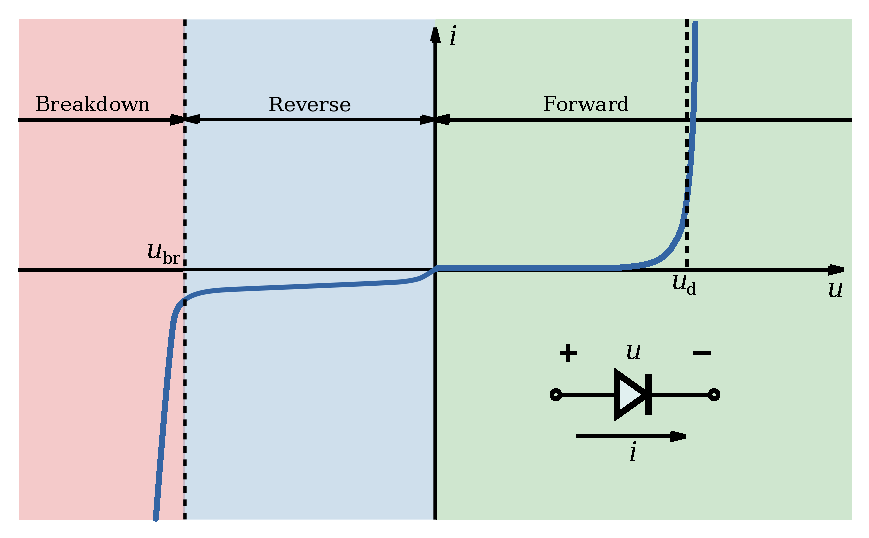
\includegraphics{images/diode-iv-curve.eps}
\label{diode-iv-curve}
\caption{Die Strom-Spannungs-Kennlinie einer LED}
\end{center}
\end{figure}
Die Strom-Spannungs-Kennlinie (Abbildung \ref{diode-iv-curve}) einer \gls{LED} zeigt recht deutlich, dass es nicht möglich ist, diese ohne externe Regelung an einer Spannungsquelle -- wie den meisten handelsüblichen Netzteilen -- zu betreiben. Eine direkt an eine niederohmige Spannungsquelle angeschlossene \gls{LED} würde sofort von einem extrem hohem Strom durchflossen werden, durch den bei gegebener \gls{Flussspannung} $\Delta U$ der \gls{LED} nach $P=U\cdot I$ eine große Leistung an der \gls{LED} anfallen würde, die die \gls{LED} erhitzen und letztlich innerhalb eines Sekundenbruchteils thermisch zerstören würde, da auch die \gls{Sperrschicht} einer Hochleistungs-\gls{LED} nicht über 150°C erhitzt werden darf\cite{PHILIPS1,PHILIPS2}.

Die zwei gängigsten Methoden der Stromregelung sind Vorwiderstände und Konstantstromquellen. Vorwiderstände werden nach $R=\frac{U}{I}$ bemessen, wobei $I$ der gewünschte Strom an der \gls{LED} ist und sich $U$ als Differenz der Betriebsspannung $V_{CC}$ und der \gls{Flussspannung} der \gls{LED}:
\begin{equation}150
R=\frac{V_{CC}-\Delta U_{LED}}{I_{LED}}
\end{equation}
Die überschüssige Leistung fällt am Vorwiderstand ab, weshalb sich diese Ansteuerung nicht für hohe Spannungsdifferenzen oder hohe Ströme eignet.
\begin{equation}
P_{R_v,tot}=\left(V_{CC}-\Delta U_{LED}\right)\cdot I_{LED}
\end{equation}
Beim Betrieb einer weißen $2,1W$-Hochleistungs-\gls{LED} mit einer Flussspannung von $3,0V$ bei $700mA$ an einer Spannungsquelle von $V_{CC}=24V$ mit Vorwiderstand fielen an diesem knapp $15W$ Verlustleistung an.
%FIXME Schaltplan
Weitere Nachteile der Verwendung von Vorwiderständen sind, dass Hochleistungswiderstände zum einen reltaiv teuer sind und zum anderen üblicherweise mit Toleranzen zwischen $5$ und $10\%$ gefertigt werden. Eine solche Toleranz stört bei der Ansteuerung einer einzelnen \gls{LED} nicht weiter, sollen jedoch mehrere \glspl{LED} als Array betrieben werden, merkt man selbst Helligkeitsunterschiede von $1\%$ bereits.

\newglossaryentry{Shunt}{name={Shunt}, description={Niederohmiger ($0.01-1\Omega$) Messwiderstand, der zur Strommessung verwendet wird. Der durch den Widerstand fließende Strom wird indirekt durch die am Widerstand abfallende Spannung gemessen. Der Widerstand sollte möglichst klein -- gegenüber dem Lastwiderstand in jedem Falle klein -- sein, um den Spannungsabfall am Widerstand und den Messfehler sowie die Verlustleistung (bei hohen Strömen) gering zu halten.}}
Alternativ und bei der Ansteuerung von Hochleistungs-\glspl{LED} weiter verbreitet ist die Konstantstromquelle. Eine Konstantstromquelle besteht aus einem Strom-Spannungs-Wandler, einem Stromregler, einer Referenz und einem Fehlerverstärker. Unabhängig von Last und Betriebsspannung sowie Innenwiderstand der Spannungsquelle stellt sich durch die Konstantstromquelle dem Namen gemäß ein sehr konstanter, von der Genauigkeit des Strom-Spannungs-Wandlers (meist ein spezieller, niederohmiger Messwiderstand -- \gls{Shunt} genannt) abhängiger Strom ein. Im Gegensatz zum Vorwiderstand lässt sich die Konstantstromquelle relativ einfach mit einem Trimmpotentiometer kalibrieren.
%FIXME Wikipedia (source/bibtex), schematics

\newglossaryentry{DAC}{name={DAC}, description={Digital Analog Converter, Digital-Analog-Umsetzer, in deutscher Fachliteratur teilweise als DAU bezeichnet}, first={Digital-Analog-Umsetzer (DAC)}, firstplural={Digital-Analog-Umsetzer (DACs)}, text={DAC}, plural={DACs}, type=\acronymtype}
\subsubsection{Dimmen - Techniken}
Das Dimmen bezeichent die Einstellung der Helligkeit der Lampe. \glspl{LED} lassen sich gut dimmen, indem man den Strom reguliert. Man kann den Strom prinzipiell analog oder digital steuern. Eine analoge Regelung besteht aus einer Modifikation der Stromquelle, im Falle der Konstantstromquelle kann dies durch ein analoges oder digitales Potentiometer\footnote{So genannte digitale Potentiometer verhalten sich genau genommen nicht wie Potentiometer. Technisch sind sie \glspl{DAC}, die einen digitalen Wert in einen Widerstand umwandeln.} oder das Inkorporieren eines einem \gls{DAC} entnommenen analogen Signals im Fehlerverstärker.
%Quellen

Beide Techniken sind relativ Störanfällig (da analoge Signale wesentlich aufmerksamerem Schaltungsdesigns bedürfen) und haben das Problem, dass \glspl{DAC} und besonders digitale Potentiometer relativ teuer sind.

\newglossaryentry{PWM}{name={PWM}, description={Pulse Width Modulation, Pulsweitenmodulation}, first={Pulsweitenmodulation (PWM)}, text={PWM}, type=\acronymtype}
\newglossaryentry{PDM}{name={PDM}, description={Pulse Density Modulation, Pulsdichtemodulation}, first={Pulsdichtemodulation (PDM)}, text={PDM}, type=\acronymtype}
Digital lässt sich eine Helligkeitsregelung durch so genannte \gls{PWM} oder \gls{PDM} erreichen. Ich werde zunächst auf die \gls{PWM} eingehen, da ihr Konzept meiner Meinung nach einfacher zu verstehen ist, um dann auf die Pulsdichtemodulation einzugehen.

\newglossaryentry{Hertz}{name={Hertz}, description={Einheit der Frequenz, entspricht nach dem SI (Système Internationale) $\frac{1}{s}$}, text={Hertz}}
%gls-entry: akzente auf S...I...?!
\subsubsection{Funktionsweise der PWM}
\glslink{PWM}{Pulsweitenmodulation} beschreibt eine Gruppe von Verfahren, bei denen die an einer Last anliegende Leistung eingestellt wird, indem die Last, die bei konstanter Stromzufuhr eine als konstant anzunehmende Leistung zeigt, mit hoher Frequenz ein- und ausgeschaltet wird. Im Konkreten Fall wird die \gls{LED} mit einer Frequenz von einigen hundert \gls{Hertz} angesteuert. Sie wird am Anfang jeder Periode der Dauer $T$ ausgeschaltet und nach einer bestimmten Zeit $t_E$ wieder eingeschaltet. Über die Periode gemittelt beträgt die Leistung der \gls{LED} $P_{LED}$ bei gegebener Volllast-Leistung $P_V$ gemittelt $P_{LED}=\frac{t_E}{T}\cdot P_{V}$. Durch die hohe Schaltfrequenz ist das die Leistung, die die \gls{LED} für ein menschliches Auge scheinbar abstrahlt.
%``leistung abstrahlen'', sprache?!
%Graphik

Eine \gls{PWM} kann überall dort zur Leistungsregelung verwendet werden, wo zwischen dem Ausgangssignal der \gls{PWM}-Steuerung und dem letztendlich durch den Aktor beeinflussten System ein Tiefpass mit einer hinreichend unterhalb der PWM-Frequenz $f_{PWM}$ liegenden Grenzfrequenz ist --- wie im Falle der \gls{LED} das Auge, das zwischen der rein technisch gesehen \glqq flackernden\grqq\ \gls{LED} und der weiteren Signalverarbeitung im Gehirn als Tiefpass mit einer Grenzfrequenz im Bereich $20$ - $30$ Hz liegt.

\newglossaryentry{Flipflop}{name={Flipflop}, description={Eine elektronische Speicherschaltung, siehe hierzu \annot{FIXME}}, text={Flipflop}, plural={Flipflops}}
\newglossaryentry{Ueberlauf}{name={Überlauf}, description={Aktion eines Zählers oder einer Variable, beim Inkrement über sein/ihr Maximum auf sein/ihr Minimum zu Springen}, text={Überlauf}, plural={Überläufe}}
%Wikipedia, etc. (Webquellen!)
Die Technische Umsetzung der Pulsweitenmodulation mit einem digitalen Eingangssignal sieht meist wie in
%Graphik!
gezeigt aus: Ein Zähler zählt von 0 zu seinem Maximum, das der Auflösung der \gls{PWM} entspricht, im Falle eines digitalen Systems üblicherweise $2^n$, wobei $n$ die Anzahl der Bits des \gls{PWM}-Steuersignals ist. Der Wert des Zählers wird durch einen digitalen Komparator kontinuierlich mit dem eingestellten Wert verglichen, und bei einem \glqq Match\grqq, also in dem Fall, dass Zählerstand und eingestellter Leistungswert übereinstimmen, wird ein ausgangsseitiges \gls{Flipflop} getriggert. Beim \gls{Ueberlauf} des Zählers wird dieses Flipflop wieder zurückgesetzt.

Die oben beschriebene \gls{PWM}-Technik ist nur eine mehrere möglicher Varianten. Da es eine große Anzahl derselben gibt und deren Theorie sehr komplex ist und diese Arbeit keine Abhandlung über Pulsweitenmodulationen sein soll, seien dem geneigten Leser die im Literaturverzeichnis aufgezählten Quellen wärmstens empfohlen \cite{ATMEL1, ATMEL2, ATMEL3}.

\subsubsection{Pulsdichtemodulation}
Bei der \gls{PDM} wird wie bei der \gls{PWM} die durchschnittliche Einschaltzeit -- im englischen \glqq on-time\grqq\ -- der Last moduliert, indem die Leistung zwischen $0\%$ und $100\%$ oszilliert. Bei der Pulsdichtenmodulation ist das Steuersignal im Gegensatz zu dem der PWM wesentlich hochfrequenter. Ein Pulsdichtenmoduliertes Signal kann analog mit einem Delta-Sigma-Modulator gewonnen werden, ein Verfahren, dass in $\Delta-\Sigma-$ADCs zum Einsatz kommt. \cite{MAXIM21, MAXIM10} Digital kann ein solches Signal durch ein digitales Modell des $\Delta-\Sigma-$ADCs generiert werden \cite{WP1, WP3}.
\begin{figure}
\begin{center}
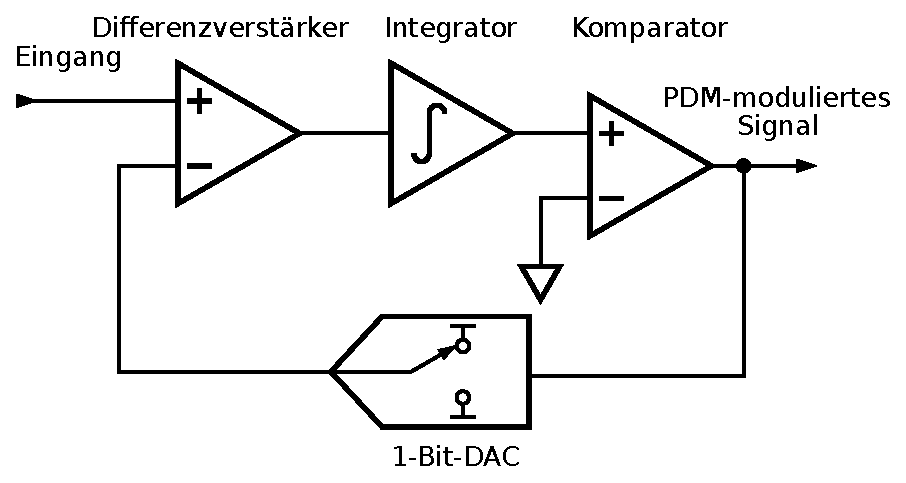
\includegraphics{images/delta-sigma-adc.eps}
\label{delta-sigma-modulator}
\caption{Schematische Zeichnung eines Delta-Sigma-Modulators}
\end{center}
\end{figure}
%Quellen, Delta-Sigma-DAC/ADC

\subsubsection{Generierung scheinbar linearer Helligkeitverläufe}
Das menschliche Auge hat eine nichtlineare Wahrnehmungscharakteristik. Nicht nur werden, wie bekannt sein sollte, verschiedene Wellenlängen mit unterschiedlicher Empfindlichkeit wahrgenommen, es werden auch verschiedene Strahlungsintensitäten mit unterschiedlicher Empfindlichkeit wahrgenommen. Der Zusammenhang zwischen realer und wahrgenommener Helligkeit ist nicht linear. Bei relativ geringer absoluter Helligkeit ist die Empfindlichkeit für kleinste Helligkeitsänderungen wesentlich größer als bei großen absoluten Helligkeiten. Zeichnet man die ungefähre Kennlinie auf ergibt sich ein logarithmischer Zusammenhang.

Effekt dieser nichtlinearen Kennlinie ist, dass eine einfache lineare Steigerung der abgestrahlten Leistung wie sie bei einer nach dem oben beschriebenen Prinzip arbeitenden \gls{PWM} durch ein Erhöhen des Leistungswertes um einen konstanten Summanden von Zyklus zu Zyklus erreicht werden könnte, in dunkleren Bereichen als wesentlich schneller ändernd als in helleren erscheint. Während die Helligkeitsänderung im Bereich maximaler Helligkeit über einen gegebenen Zeitraum als nichtexistent erscheinen kann, dimmt dieser Algorithmus im gleichen Zeitraum von $0\%$ auf scheinbar halbe Helligkeit.

\begin{figure}
\begin{Verbatim}[commandchars=\\\{\},codes={\catcode`\$=3\catcode`\^=7\catcode`\_=8}]
\PY{c+c1}{#!/usr/bin/env ruby}

\PY{n}{inbits} \PY{o}{=} \PY{l+m+mi}{8}
\PY{n}{outbits} \PY{o}{=} \PY{l+m+mi}{16}

\PY{n+nb}{puts} \PY{o}{<<}\PY{n+no}{eos}
\PY{l+s+sh}{/* }
\PY{l+s+sh}{* Logarithmic #\PYZob{}outbits\PYZcb{}-bit pwm #\PYZob{}inbits\PYZcb{}-bit lookup table}
\PY{l+s+sh}{* }
\PY{l+s+sh}{* Copyright 2010 by Jan Sebastian Götte (s@twopi.eu)}
\PY{l+s+sh}{*  - - - - - - - - - - - - LICENSE INFORMATION - - - - - - - - - - - -}
\PY{l+s+sh}{* This program is free software: you can redistribute it and/or modify}
\PY{l+s+sh}{* it under the terms of the GNU General Public License as published by}
\PY{l+s+sh}{* the Free Software Foundation, either 1.1 3 of the License, or}
\PY{l+s+sh}{* (at your option) any later 1.1.}
\PY{l+s+sh}{* }
\PY{l+s+sh}{* This program is distributed in the hope that it will be useful,}
\PY{l+s+sh}{* but WITHOUT ANY WARRANTY; without even the implied warranty of}
\PY{l+s+sh}{* MERCHANTABILITY or FITNESS FOR A PARTICULAR PURPOSE.  See the}
\PY{l+s+sh}{* GNU General Public License for more details.}
\PY{l+s+sh}{* }
\PY{l+s+sh}{* You should have received a copy of the GNU General Public License}
\PY{l+s+sh}{* along with this program.  If not, see <http://www.gnu.org/licenses/>.}
\PY{l+s+sh}{*  - - - - - - - - - - - - - - - - - - - - - - - - - - - - - - - - - -}
\PY{l+s+sh}{*}
\PY{l+s+sh}{*/}

\PY{l+s+sh}{#ifndef \PYZus{}\PYZus{}GENERATED\PYZus{}PWM\PYZus{}LUT\PYZus{}LOG\PYZus{}#\PYZob{}inbits\PYZcb{}\PYZus{}#\PYZob{}outbits\PYZcb{}\PYZus{}\PYZus{}}
\PY{l+s+sh}{#define \PYZus{}\PYZus{}GENERATED\PYZus{}PWM\PYZus{}LUT\PYZus{}LOG\PYZus{}#\PYZob{}inbits\PYZcb{}\PYZus{}#\PYZob{}outbits\PYZcb{}\PYZus{}\PYZus{}}

\PY{l+s+sh}{#include <avr/pgmspace.h>}

\PY{l+s+sh}{const uint16\PYZus{}t log\PYZus{}pwm\PYZus{}lut[] PROGMEM = \PYZob{}}
\PY{l+s+sh}{#\PYZob{}(0...2**inbits).map \PYZob{}|i| (2.0**(i/(2**inbits.to\PYZus{}f)*outbits)).round \PYZcb{}.join(", ")\PYZcb{}}
\PY{l+s+sh}{\PYZcb{};}

\PY{l+s+sh}{#endif//\PYZus{}\PYZus{}GENERATED\PYZus{}PWM\PYZus{}LUT\PYZus{}LOG\PYZus{}#\PYZob{}inbits\PYZcb{}\PYZus{}#\PYZob{}outbits\PYZcb{}\PYZus{}\PYZus{}}

\PY{n+no}{eos}
\end{Verbatim}

\caption{Ein Ruby-Script, dass auf Basis dieser Formel eine C-Headerdatei mit einer Lookup-Tabelle für alle Eingabehelligkeitswerte generiert}
\end{figure}

Abhilfe für diesen Umstand lässt sich durch die Transformation eines rohen Helligkeitswertes, der der optisch wahrgenommenen Helligkeit entspricht nach einer logarithmischen Skala auf den Wertebereich der \gls{PWM}. Dies kann z.B.\ nach folgender Formel geschehen:
\begin{equation}
2^{\left(\frac{v}{2^n}\cdot k\right)}
\end{equation}
\begin{align}
v&:=\text{Eingabewert auf einer linearen Skala}\\
n&:=\text{\glqq Breite\grqq\ des Eingabewertes in Bit}\\
k&:=\text{\glqq Breite\grqq\  des Ausgabewertes in Bit}
\end{align}
Hierzu siehe auch \cite{MAXIM41,MAXIM57,SIART1}.
%Diagramm

\subsubsection{Umsetzung}
Für das Dimmen der Hochleistungs-LEDs verwende ich in der ersten Version des Prototyps eine Kombination aus analog geregelter Konstantstromquelle, die den für den Dauerbetrieb maximal möglichen Strom von ca. 330mA pro Kanal/LED einstellt und der Modulation per 16-Bit-PWM von einem AVR-Mikrocontroller gesteuert. Für Details der Pulsweitenmodulation ist das Datenblatt der AT90PWM-Reihe sehr hilfreich, da dieser speziell für solcherlei Einsatzzwecke designt wurde\cite{ATMEL2}. Die konkret verwendeten Controller sind in der ersten Version der Steuerplatine zwei ATMega8-AVRs zuständig, die jeweils über zwei 16-bit-PWM-Kanäle verfügen und die per serieller Schnittstelle (TTL-Pegel) koordiniert werden. Die Auflösung der PWM habe ich auf 16 Bit festgelegt, da die benötigte logarithmische Kurve bei einer 8-Bit-PWM erkennbare Abstufungen zeigt. Die Firmware unterstützt mit dem im vorherigen Abschnitt %TODO NOTE: this could be incorrect since the arrangement could be changed.
generierte Tabellen in nur durch die auf 16 Bit beschränkte Ausgangsauflösung und den im AVR nur begrenzt vorhandenen Programmspeicher, in dem die Tabellen abgelegt würden, eingeschränkte Eingabebitbreiten. 12 Bit haben sich hier als sinnvoll erwiesen, da sie auch bei %``da sie'' oder ``da dies''
niedrigen Helligkeitseinstellungen keine Stufen sichtbar werden lassen.

Revision 2 der Prototypenhardware sieht einen ATMega16U4-Mikrocontroller vor, der über vier nutzbare 16-Bit-PWM-Kanäle verfügt und somit die Serielle Koordination beider Prozessoren überflüssig macht. Außerdem verfügt er neben zwei seriellen Schnittstellen (die zur Kommunikation mit anderen Systemen genutzt werden) auch über eine USB-Schnitstelle, sodass die Lampe auch direkt an einen modernen Computer angeschlossen werden kann.

Für Revision 3 der Prototypenhardware habe ich eine rein \glqq digitale\grqq\ Stromregelung geplant. Diese bestünde aus einem Step-Down-Wandler (Buck Converter),%Note: Literature!!!, Glossary.
der durch eine vom AVR generierte 16-Bit-PWM angesteuert wird. Der Strom durch die LED wird mit einem der in den AVR-µC integrierten 10-Bit-ADCs gemessen. Das Messignal wird aus dem Spannungsabfall über einen Shunt%glossary
mit einem logarithmischen Differenzverstärker generiert.

\subsection{Kommunikationsprotokoll}
Zur Kommunikation verschiedener Beleuchtungsmodule untereinander entwickelte ich einen Bus mit dem Namen BUZ2, der auf Basis eindeutiger 16-bittiger Geräteadressen durch einen Master koordinierte, kollisionsfreie Kommunikation auf einem RS485-Bus erlaubt. Das Kommunikationsprotokoll ist paketbasiert, wobei Pakete durch vom Master ausgesendete Escapesequenzen eingeleitet werden. Die Verwendung solcher Escapesequenzen erspart die Verwendung eines dedizierten Steuerkanals oder eines neunten Datenbits um Kommandos zu markieren. Ein an den Bus angeschlossenes Gerät kann eine Transaktion nicht selbstständig beginnen, stattdessen wird es periodisch mvom Master adressiert. Nach dem Standardalgorithmus wird es so lange erneut adressiert, bis es keine zu übertragenden Daten mehr in der Queue hat. Bisher stellte dieses Verhalten kein Problem dar, sollte das Bussystem jedoch später für größere Netzwerke Verwendung finden, wäre hier ein intelligenterer Scheduling-Algorithmus angebracht. Die Datenintegrität wird durch eine CRC-16-Prüfsumme sichergesteellt. Kann der Empfänger ein Paket nicht als fehlerfrei empfangen quittieren wird der Sendevorgang bis zum Erreichen einer einstellbaren maximalen Anzahl der Versuche wiederholt.

Die Software ist in C für AVR-Mikrocontroller geschrieben, sollte jedoch relativ einfach auf andere Plattformen portierbar sein insofern diese C oder Assembler bzw.\ eine andere Sprache, zu der sich C einfach konvertieren lässt wie Java unterstützen. Das Softwaremodul kann in jede Anwendung einkompiliert werden und es ist möglich, Kommandos selbst nach Belieben zu spezifizieren.

\subsubsection{Master}
Der Master ist das einzige Device auf dem Bus, das eigenständig Transaktionen beginnen darf. Der Master gibt für die Pakete aller anderen Devices di\glqq Rahmen\grqq\ vor und adressiert reihum das jeweils sendende Device. Der Master übernimmt zudem die Entdeckung neuer Devices mit einem speziellem Paket, dem \glqq Discovery Packet\grqq.
\subsubsection{Slave}
\subsection{Kompatible Steuergeräte}
\section{Grundlagen der Elektroenzephalographie}
\subsection{Biologisch}
\subsection{Elektrisch}
Hirnströme lassen sich auf der Kopfhaut noch mit einer Amplitude von ca.\ $10-100µV$ messen\cite{MAYER1}. Die Messung solcher Spannungen ist kein allzu einfaches Unterfangen. Problematisch an der Messung solch kleiner Hirnströme ist noch, dass durch den hohen scheinbaren Innenwiderstand die zur Messung nutzbare Stromstärke extrem gering ist ($nA$-Bereich) und somit der Innenwiderstand der Messschaltung extrem hoch sein muss.

%TODO gls entry
\newglossaryentry{Fehlerstrom}{name={Fehlerstrom}, description={Unerwünschter, häufige gefährlicher, auf nicht intendiertem Wege fließender Strom, meist durch Lebewesen}}
Da an besagter Messschaltung ein Mensch angeschlossen ist\footnote{dessen Schaltbild in eingängiger Fachliteratur tatsächlich ein Strichmännchen ist} sind besondere---wiewohl nicht unbedingt notwendige---Schutzschaltungen einzuplanen. In der konkreten Umsetzung sind das einige $100k\Omega$-Schutzwiderstände, die den maximalen \gls{Fehlerstrom} auf unbedenkliche Werte begrenzen.
%Graphik/Schaltplan

%Schaltplan
\newglossaryentry{ADC}{name={ADC}, description={Analog Digital Converter, Analog-Digital-Umsetzer, in deutscher Fachliteratur teilweise als ADU bezeichnet}, first={Analog-Digital-Umsetzer (ADC)}, firstplural={Analog-Digital-Umsetzer (ADCs)}, text={ADC}, plural={ADCs}, type=\acronymtype}
Den Teil des \gls{EEG}, der die Messsignale von den Elektroden in digitale Signale zur Weiterverarbeitung umwandelt wird als \glqq analoges Front-End\grqq\ bezeichnet. Das analoge Front-End eines \gls{EEG} sieht prinzipiell folgendermaßen aus: Auf die Elektroden folgt zunächst eine Schutzschaltung, die verhindert, dass auf den Benutzer des Gerätes bedenkliche Spannungen respektive Ströme einwirken. Auf diese Schutzschaltung folgt der Vorverstärker, der das Messsignal konditioniert und auf ein zur Weiterverarbeitung fähiges Spannungslevel bei geringem Spannungsquelleninnenwiderstand transformiert. Im Vorverstärker integriert sowie unmittelbar dahinter folgen analoge Filter, die das Signal auf die für die weitere Analyse interessante Bandbreite reduzieren. Schließlich folgt noch der \gls{ADC}, durch den die abschließende Umwandlung des aufbereiteten Messsignals in eine Folge digitaler Werte erfolgt.

\newglossaryentry{IC}{name={IC}, description={Integrated Circuit, Integrierter Schaltkreis, umgangssprachlich Mikrochip}, first={Mikrochip (IC)}, firstplural={Mikrochips (ICs)}, text={IC}, plural={ICs}, type=\acronymtype}
Das analoge Front-End meiner \emph{OpenMind} getauften Eigenentwicklung enthält als zentrales Element einen speziell für die Anwendung in \glspl{EEG} entwickelten \gls{IC}. Der ADS1194 des Herstellers Texas Instruments enthält analoge Filter, Vorverstärker und ADC\cite{TEXAS1}. Der in meinem Design eingesetzte ADS1194 enthält 4 Eingangsschaltungen und wird in meinem Design eingesetzt, um die Signale von bis zu vier Elektroden aufzunehmen.

\begin{landscape}
\begin{figure}
\begin{center}
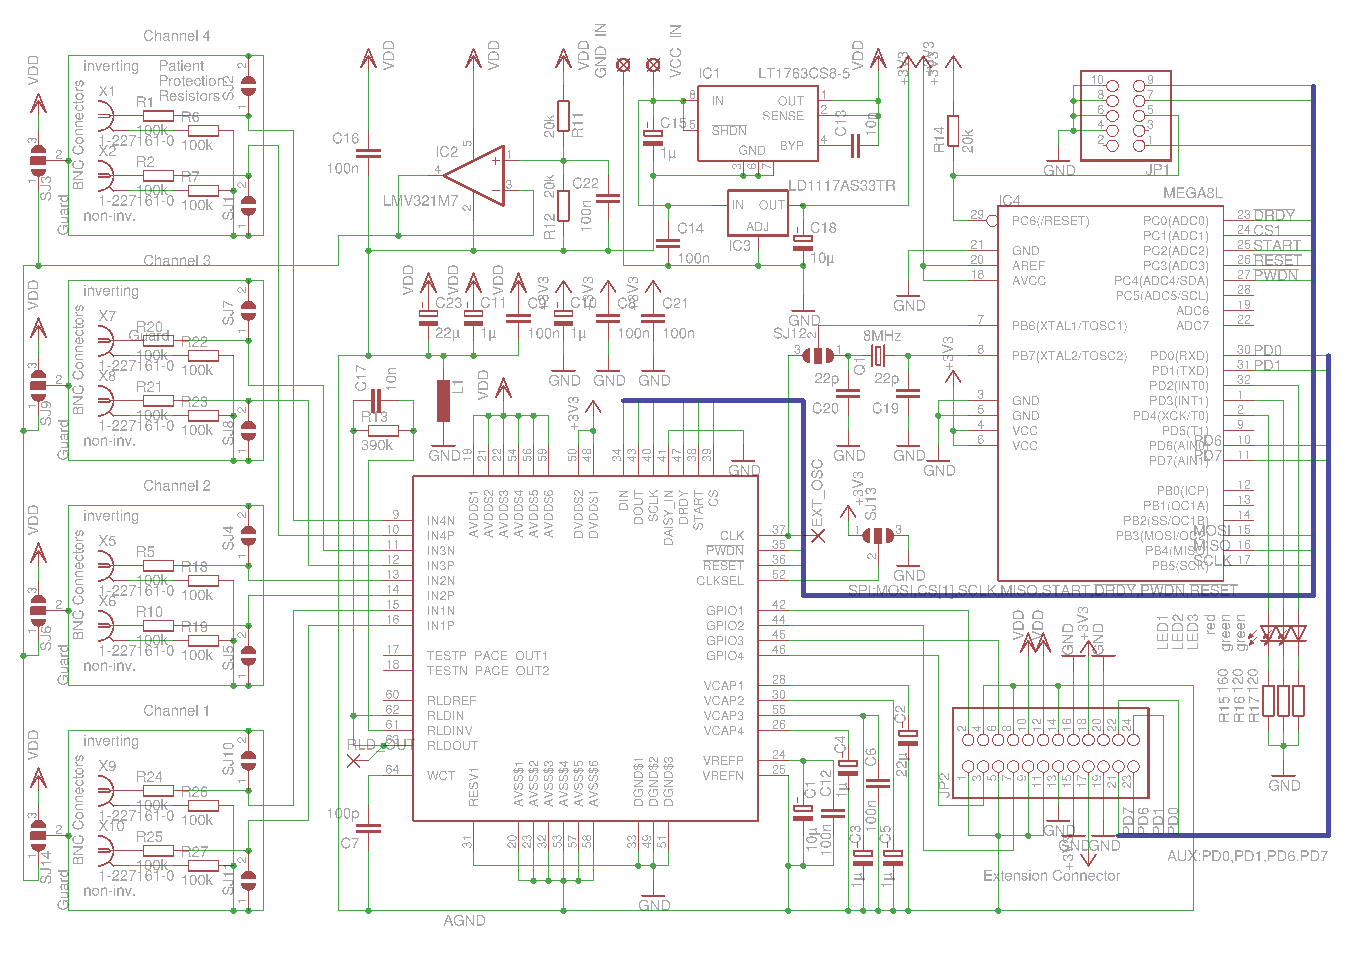
\includegraphics{images/adc_schematic_01.eps}
\label{adc_schematic}
\caption{Der Schaltplan des EEG-Moduls}
\end{center}
\end{figure}
\end{landscape}

\newglossaryentry{Sampling}{name={Sampling}, description={Umwandlung eines kontinuierlichen, meist analogen Signals in diskrete Werte und -- im Falle eines ADC oder DAC -- die Umwandlung desselben in digitale Signale}}
\newglossaryentry{Nyquist-Theorem}{name={Nyquist-Theorem}, description={}}
\newglossaryentry{Offsetkorrektur}{name={Offsetkorrektur}, description={}}
%TODO: gls entries
Die \gls{Sampling}-Rate liegt im Bereich einiger hundert bis tausend $\frac{Sp}{s}$, die höchste für die Messung signifikante Frequenz liegt weit unter $100Hz$. Das \glslink{Nyquist-Theorem}{Nyquist-Shannonsche Abtasttheorem} ist somit erfüllt und bei den gegebenen Frequenzen sind keine Probleme zu erwarten.
Die Auflösung des \gls{ADC} ist mit 16 Bit groß genug, um \gls{Offsetkorrektur} und weitere Filtermaßnahmen in Software zu implementieren, wodurch keine weiteren analogen eingangsseitigen Filter notwendig sind.
%Quelle: Nyquist

%BEGIN OF TODOS
% --- PAPER ---
%Include: in the PWM section: Duty cycle
%Bildquellenverzeichnis
% --- SOURCES ---
%AN4348 Pg. 5: Error? The tolerance calculation seems to be mixing up ppms and percents.
% --- ELECTRONICS ---
%Incorporate a MAX5490 or similar calibrated R-R ladder as reference voltage divider
%Input decoupling necessary?
%END OF TODOS
\newglossaryentry{FFT}{name={FFT}, description={FIXME}}
\subsection{Mathematisch und Informatisch}
Die Auswertung der Messergebnisse kann auf verschiedene Arten geschehen. Da die Messelektronik noch nicht vollständig läuft, habe ich noch keinen Algorithmus umgesetzt.
Grundsätzlich bietet es sich an, das Messignal z.B.\ mit einer \gls{FFT} in den Frequenzraum zu übertragen. Zur Erkennung der 
\cite{WP2,WP11,WP12,WP13}
\section{Arbeitsprozess der Platinenherstellung und Ergebnisse}
\appendix
\section{Glossar}
%FIXME
\glsaddall
\printglossaries
\section{Literatur, Quellen etc.}
\nocite{*}
\bibliographystyle{plain}
\renewcommand{\refname}{}
%TODO \footnotesize
\bibliography{rgbulb}
\section{Updates}
\begin{center}
\Ovalbox{
\begin{minipage}{11cm}
\begin{center}
\sffamily%\color{red}
\vspace{2mm}
Die jeweils aktuellte Version dieser Arbeit, der Quelltexte und der Hardwaredokumentation ist unter der Adresse 
\url{http://github.com/jaseg/RGBulb} zu finden. Die Repositories der einzelnen Unterprojekte sind unter den folgenden Adressen zu finden:
\begin{description}
\item \url{https://github.com/jaseg/OpenMind}
\item \url{https://github.com/jaseg/BUZ2-Master}
\item \url{https://github.com/jaseg/BUZ2-Slave}
\end{description}
\vspace{2mm}
\end{center}
\end{minipage}
}
\end{center}
\section{Changelog}
\begin{tabularx}{\textwidth}{l|l}
\textbf{Version}&\textbf{Anmerkungen}\\\hline
0.1&Arbeitsversion
\end{tabularx}
\end{document}